\section{Hjertets overordnet anatomi og fysiologi}\label{Hjerte_ana_fys}

Hjertets primære funktion er at transportere blod, der indheolder ilt og næringsstoffer, rundt i kroppen. Det er derfor et essentielt organ for kroppen, hvilket tydeliggør sig f.eks. ved at hvis hjertet holder op med at slå, vil den pågældende person miste bevidstheden allerede efter 5-10 sekunder \cite{gronanatomi}. Hos et voksent menneske, er hjertet omtrent lige så stort som en knyttet hånd, og vejer ca. 300-350 gram for mænd, hvorimod kvinders hjerte har en vægt på omtrent 250-300 gram. Hjertet er placeret mellem højre og venstre lunge, bag sternum i thoraxhulen som ses på figur \ref{fig:hjerte_placering}. 

\begin{figure}[H] % Example of including images
\begin{center}
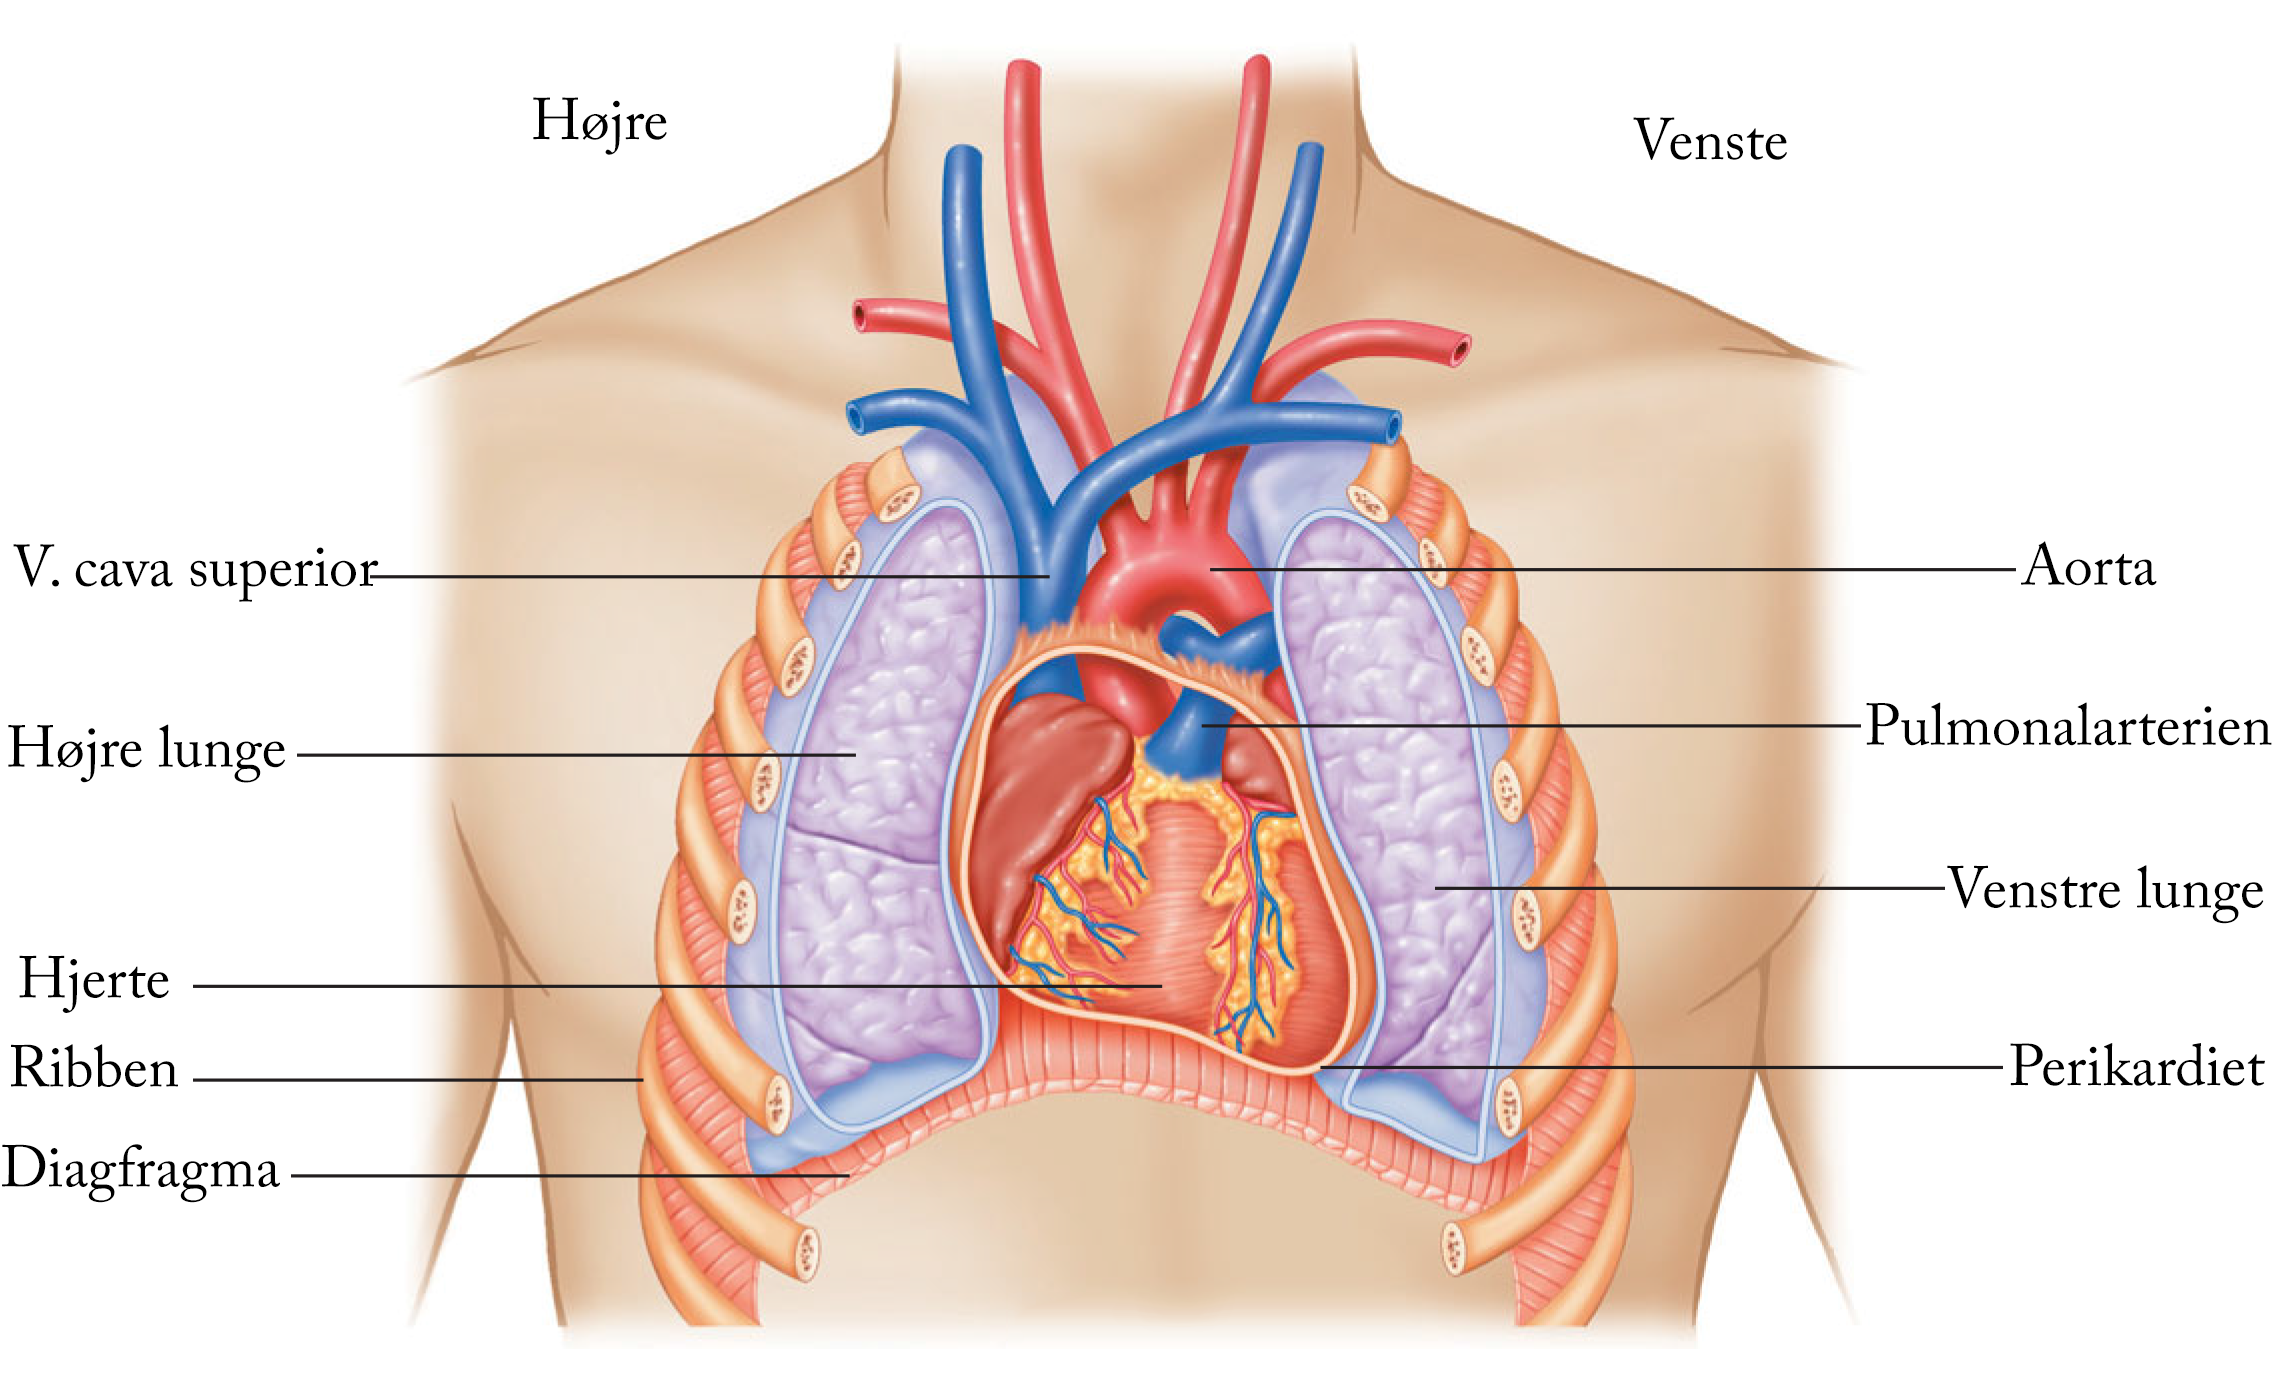
\includegraphics[width=1\textwidth]{figures/thorax}
\end{center}
\caption{Illustration af hjertets placering i thoraxhulen. \cite{cindy}}
\label{fig:hjerte_placering}
\end{figure}

\noindent Hjertet er omgivet af en tynd hinde, perikardiet, som består af kollagene fibre. Laget er med til at stabilisere hjertet og dets tilhørende blodkar i mediastinum, og med til at smøre hjertet for at nedsætte friktionen. Hjertet fungerer som en pumpe, der pumper blod rundt i hele kroppen vha. trykforskelle med et interval bestemt af hjertets elektriske signal. Disse trykforskelle opstår fordi hjertet er et hult muskelorgan med fire kamre; højre og venstre atrium, og højre og venstre ventrikel samt en række klapper til at holde blodet inde eller ude. Dette er illustreret på figur \ref{fig:hjerte_overordnet}.

\begin{figure}[H] % Example of including images
\begin{center}
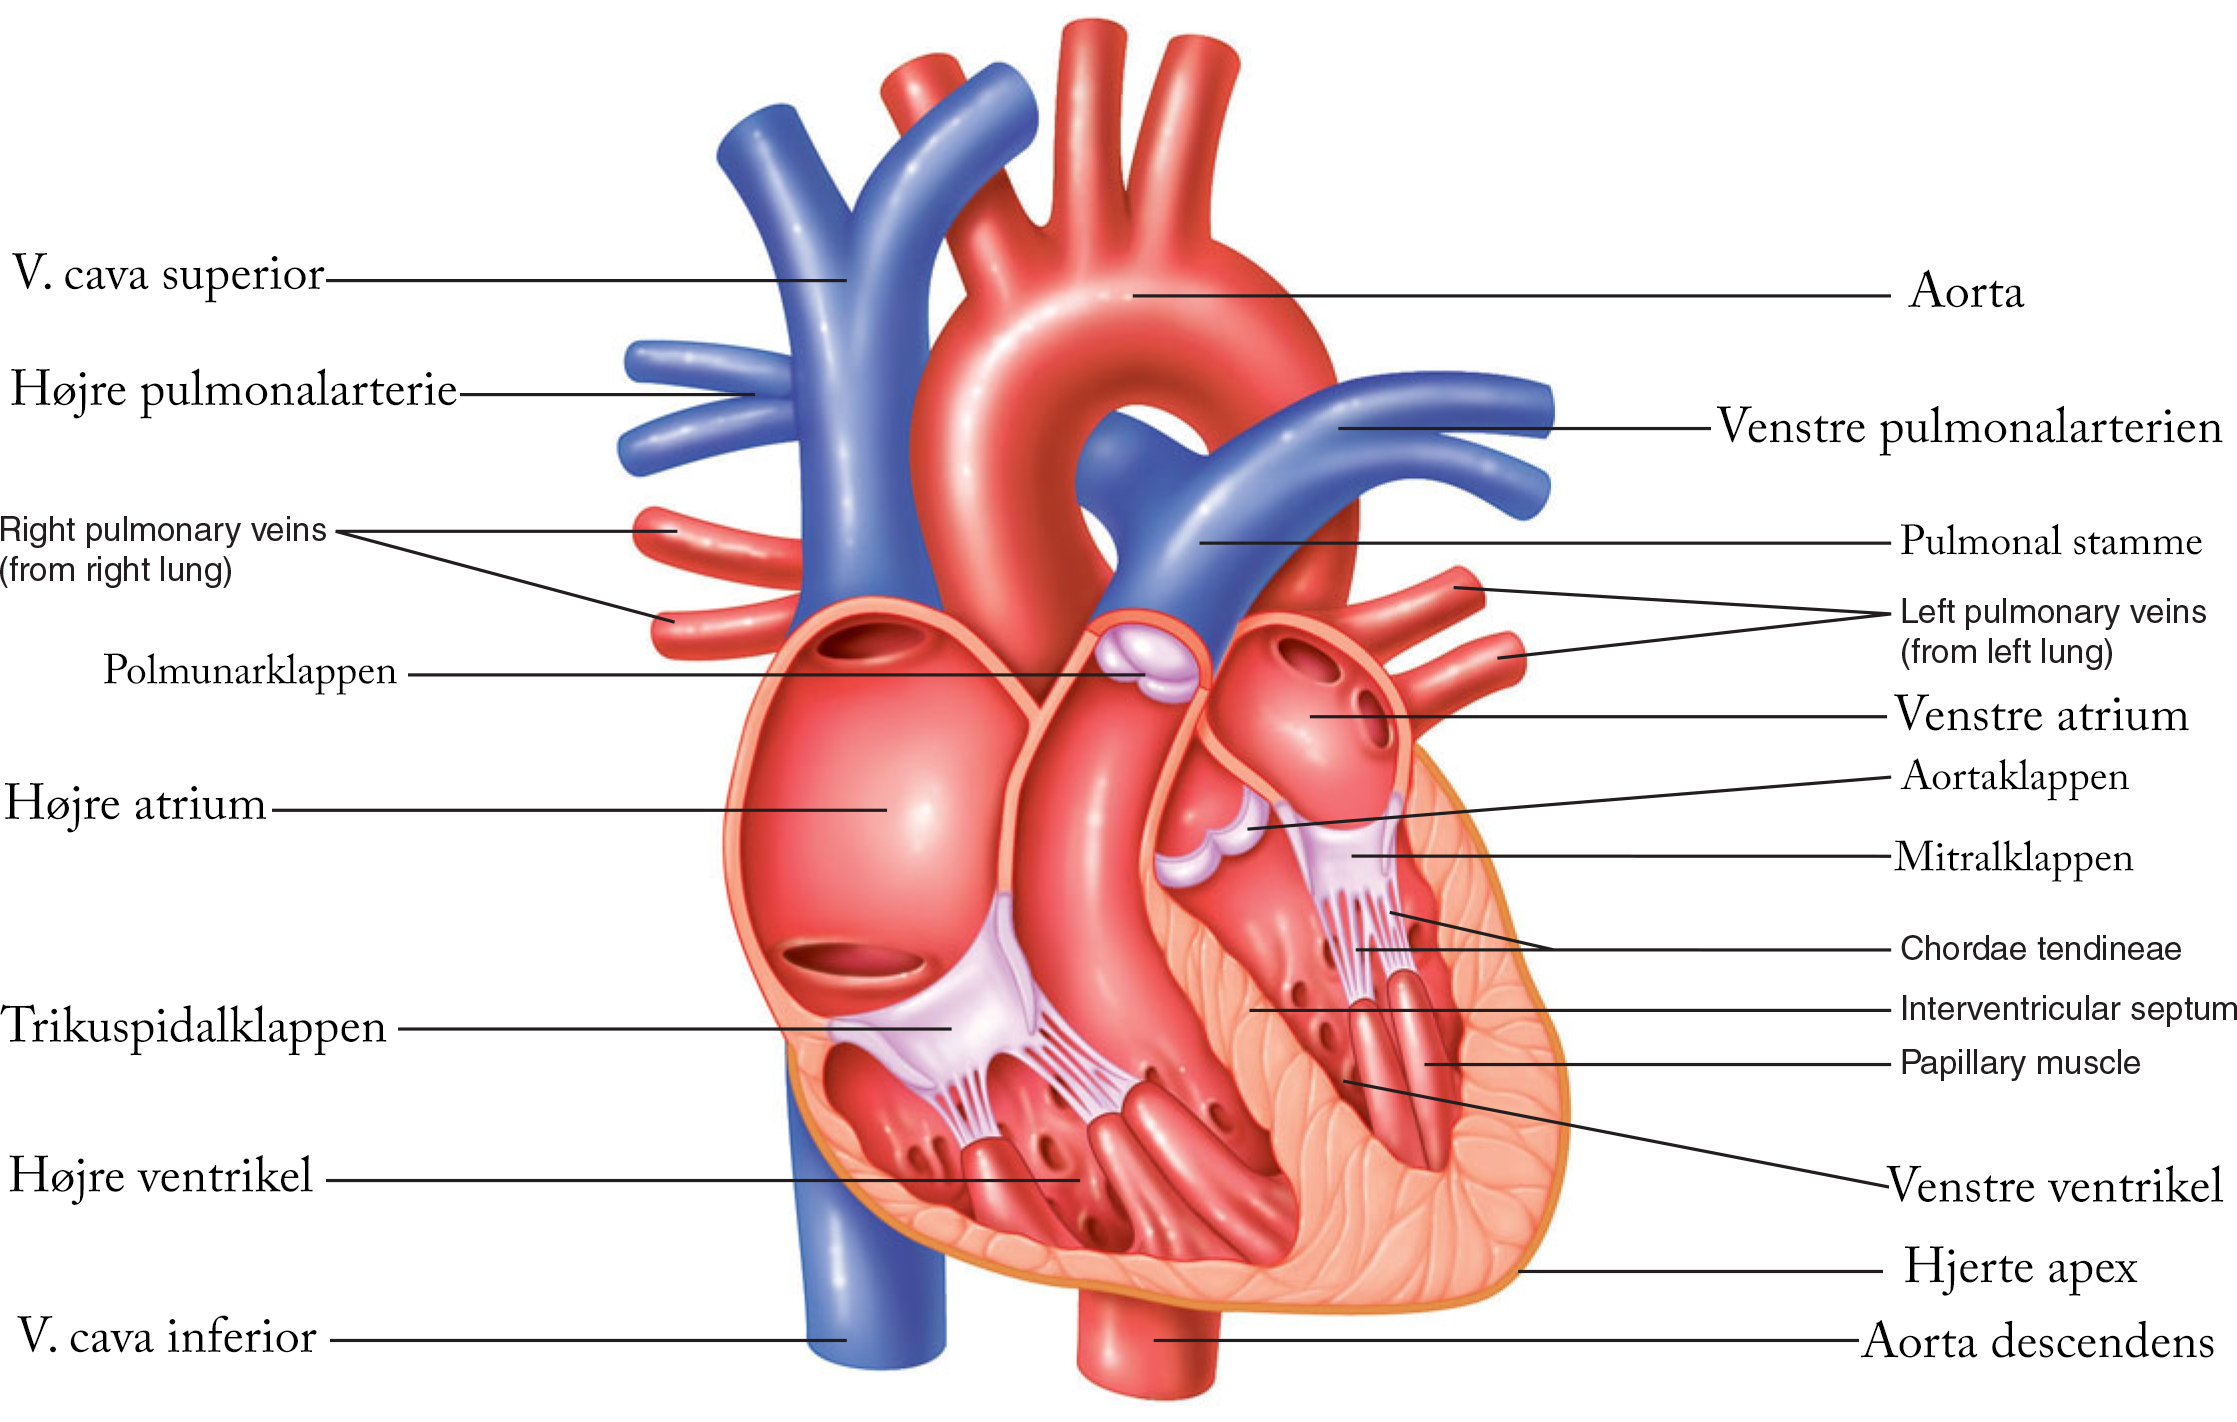
\includegraphics[width=0.5\textwidth]{figures/hjertet_overordnet}
\end{center}
\caption{Illustration af hjertets overordnet anatomiske opbygning \cite{Guyton2006}}
\label{fig:hjerte_overordnet}
\end{figure}


\noindent Hjertevæggen er opbygget af tre lag; endokardiet, myokardiet og epikardiet. Myokardiet er det midterste lag i hjertevæggen og dette lag udgøre hjertets muskelvæv \cite{gronanatomi}. Hjertevæv består hovedsagligt af disse celler, og disse udfører hjertets gentagne kontraktioner, hvor hjertevæggen bevæger sig indad \cite{cindy}. 
Det der kendetegner hjertemuskelceller er blandt andet at de forgrenede, de besidder kun en enkelt cellekerne pr. celle og imellem cellerne er indskudsskiver der kan fører aktionpotentialerne videre \cite{martini}.

\subsection{Hjertets klapper}
For at blodet skal strømme i den rigtige retning, har hjertet fire klapper; atrioventrikulærklapperne, som består af trikuspidalklappen, (mellem højre atrium og ventrikel), mitralklappen (mellem venstre atrium og ventrikel) og semilunærklapperne aorta- samt polmunarklappen. Semilunærklappernes funktion er at forhindre reflux af blodet til henholdsvis venstre og højre ventrikel som illustreres på figur \ref{fig:hjerte_klap}.  \cite{gronanatomi}  

\begin{itemize} 
	\item Atrioventrikulærklapperne
		\begin{itemize} 

			\item Trikuspidalklappen, (mellem højre atrium og ventrikel)
			\item Mitralklappen (mellem venstre atrium og ventrikel)

		\end{itemize} 

	\item Semilunærklapperne
		\begin{itemize} 

			\item Aortaklappen
			\item Polmunarklappen

		\end{itemize} 		
\end{itemize} 


\begin{figure}[H] % Example of including images
\begin{center}
\includegraphics[width=1\textwidth]{figures/cusp}
\end{center}
\caption{Illustration af klappernes funktion med eksempel af aorta klappen \cite{cindy}.}
\label{fig:hjerte_klap}
\end{figure}

\subsection{Hjertets blodforsyning}
Omkring 4\% af hjertets minutvolumen går igennem koronararteriene som forsyner hjertet, på trods af at hjertet kun udgør ca. 0,4\% af den samlede legemsvægt \cite{gronanatomi}. Hjertemuskelceller stiller høje krav til tilførelse af ilt og næringsstoffer ift. til de fleste andre væv i kroppen. Hjertet er nemlig ikke i stand til, på samme måde som andre væv, at udføre anaerob metabolisme derfor bruger hjertet mere end 70\% af den ilt der tilføres af hjertets egen blodforsyning. Under anstrengelse kan blodgennemstrømningen i hjertet stige til det 9 dobbelte ift. når kroppen befinder sig i hvile \cite{martini}. Koronararterierne afgår fra aorta tæt på aortaklappen. Højre del af hjertets blod forsynes hovedsageligt af a. coronaria dextra, og a. coronaria sinistra forsyner hovedparten af den venstre side af hjertet. se på figur \ref{fig:hjerte_overordnet}. Ramus interventricularis anterior som er beliggende på den anterior del af hjertet forsyner de forreste dele af ventrikelskillevæggen og de dele der støder op til denne \cite{gronanatomi}.

\subsection{Hjertets cyklus}
Hjertets cyklus repræsenterer alle begivenheder i forbindelse med gennemløb af blod i løbet af et hjerteslag. Generelt kan hjertet befinde sig i to tilstande; systole (ventriklerne er kontraherede) og diastole (ventriklerne er afslappede). Atrierne kontraheres samtidig, og ligeledes kontraheres ventriklerne samtidig. Dog vil trykket i den højre halvdel kun opnå ca. 20\% af det maksimale tryk der opnåes i venstre ventrikel. Dette skyldes at den højre halvdel kun skal pumpe blod ud til pulmonalkredløbet, hvorimod at den venstre side har til opgave at pumpe blod rundt i det systemiske kredsløb. En mere detaljeret gennemgang af hjertetscycklus kan beskrives ved at opdele cyklussen i fire faser. Disse er 1) ventrikulær fyldning, 2) isovolumisk kontraktion, 3) ventrikulær ejection og 4) isovumetrisk relaxtion.

\paragraph*{Ventrikulær fyldning}
I den første tredjedel del af denne fase vil blodet hurtigt strømme ned i ventriklerne på grund af den opståede trykforskel efter systolen. I den sidste tredjedel af denne fase, vil atrierne kontrahere, og dermed pumpe blod i ventriklerne. Denne andel svarer til at ca. 20\% af den akummulerede blodmængde i ventriklerne. 

\paragraph*{Isovolumisk kontraktion}
Det tager ca. 0,02 til 0,03 sekunder før ventriklerne har opbygget et tilstrækkeligt stort tryk til at åbne semilunærklapperne. Det vil sige at der sker en kontraktion, men der vil ikke løbe blod hverken fra eller til ventriklen pga. alle hjerteklapper er lukket i denne fase. Dette betyder at volumen ændrer sig ikke synderligt, men trykket vil blive forøget. Preload er det stræk der opstår i muskelfibrene i denne fase, og bestemmes af trykket og mængden af blod der findes i venstre ventrikel i slutningen af systolen. Preload er bl.a. med til at bestemme størrelsen på slagvolumen.

\paragraph*{Ventrikulær ejection}
Når trykket i venstre ventrikel stiger til over ca. 80 mmHg (for et normalt menneske), vil SA-klapperne åbne. Ca. 70\% af blodet tømmes i løbet af den første tredjedel af systolen. Derfor kaldes denne periode for “rapid ejection”. Den resterende periode kaldes for “slow ejection”.

\paragraph*{Isovolumetrisk afslapning}
I slutningen af systole vil den ventrikulære afslapning ske pludseligt, hvilket betyder at trykket også ændrer sig pludseligt. Blodet fra arteriene skubbes tilbage og AV-klapperne lukker. I ca. 0,03 til 0,06 sekunder vil ventrikelmusklerne blive ved med at være  afslappet, selvom volumen ikke ændrer sig \cite{guyton} \cite{cindy} \cite{gronanatomi}. 

\noindent De forskellige faser er illustreret på figur \ref{fig:hjerte_cyklus}.\\


\begin{figure}[H] % Example of including images
\begin{center}
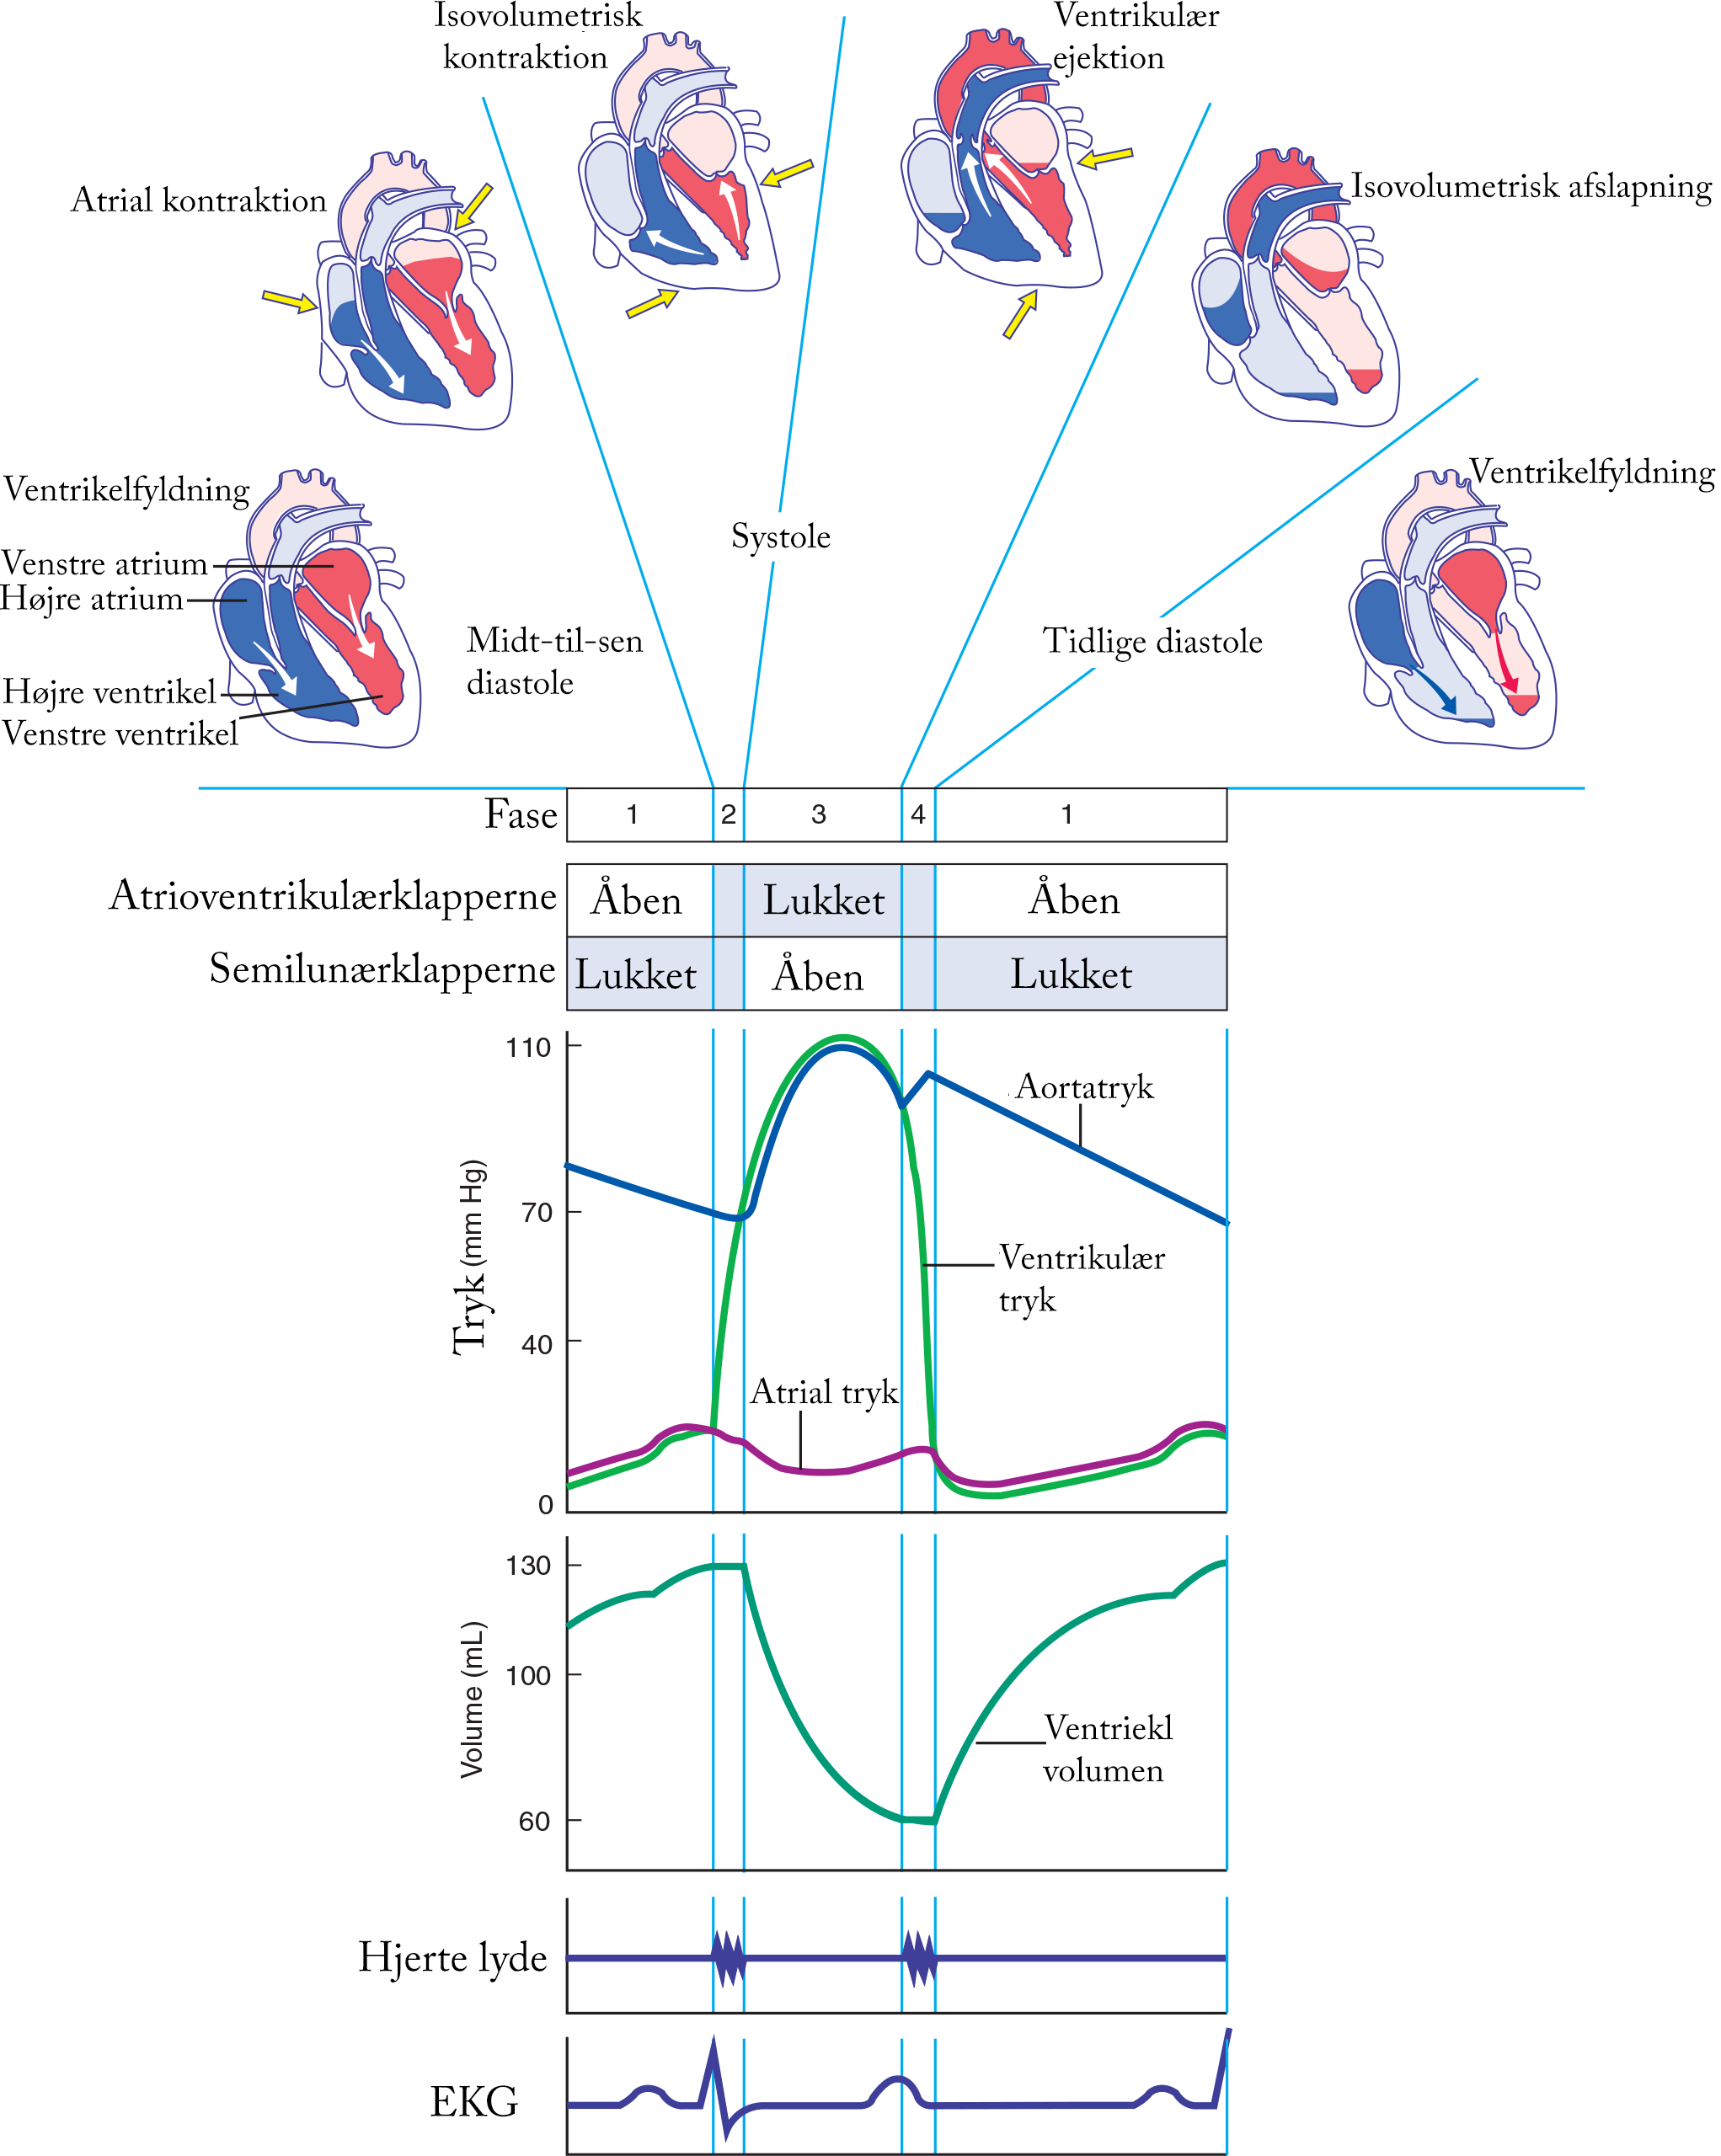
\includegraphics[width=1\textwidth]{figures/cyklus}
\end{center} 
\caption{Illustration af hjertets cyklus \cite{cindy}.}
\label{fig:hjerte_cyklus}
\end{figure}


\subsection{Hjertets elektriske ledningssystem}\label{Hjertets_elektriske_ledningssystem}
Hjertets rytmiske kontraktioner som får blodet til at pumpe rundt udføres vha. hjertets elektriske ledningssystem. Hjertemuskulaturen har den specielle evne, at den kan kontrahere sig selv uden at modtage et nervesignal \cite{gronanatomi}. Hjertet er også forsynet med sympatiske og parasympatiske nerver, og disse er med til at regulere hjerterytmen \cite{cindy}. Hjertets ledningssystem består af SA-knuden(sinus knuden),av-knuden, det His'ske bundt, grenbundterne og purkinjefibrene disse er illustreret på figur \ref{fig:hjerte_elektriske}. Aktionspotentialer der får hjertet til spontant at kontrahere, og dermed bestemme hvilken frekvens hjertet slår med, initieres i SA-knuden, og derfor bærer cellerne i SA-knuden også navnet "pacemaker" celler. SA-knuden er beliggende i den øverste del af højre atrium og cellerne i SA-knuden vil typisk fyre 60 til 100 gange i minuttet, men dette er stærkt afhængigt af det autonome nervesystems aktivitet, samt kroppens behov for at øge hjertets
minutvolumen \cite{ekgbook}.

\begin{figure}[H] % Example of including images
\begin{center}
\includegraphics[width=0.8\textwidth]{figures/hjerte_elektrisk}
\end{center}
\caption{Illustration af hjertets eleketriske system\cite{cindy}.}
\label{fig:hjerte_elektriske}
\end{figure}

\noindent SA-knudens signal føres fra celle til celle via gap junctions \cite{gronanatomi}. Disse gap-junctions muliggør en hurtig diffussion af ioner \cite{guyton}. AV-knudens primære opgave er at  forsinke det elektriske signal. Ved et normalt fungerende hjerte vil atrierne kontrahere ca. en en sjettedel af sekund før ventriklerne, og dette er fordi ventriklerne skal have mulighed for at forsynes med en tilstrækkelig mængde blod \cite{guyton}. Det His'ske bundt der fører signalet gennem anulus fibrosus som er den eneste elektriske forbindelse mellem atrierne og ventriklerne, derefter går His'ske bundt over i grenbundterne der fører signalet videre. Purkinjefibrene leverer signalet til det ventrikulære myokaridum og disse fibre har den egenskab at de kan lede de elektriske signalet hurtigt. Indenfor 75[ms] er ventriklernes væg depolariseret. Hele depolariseringsprocessen strækker sig ca. over 225[ms]\cite{gronanatomi}.



